The developed system incorporates all the standard components needed for supervised machine learning, which were described in details in the theoretical section. First of all, to perform any task concerning image processing, a dataset of images is needed. In the thesis, all required images were artificially generated. Thus, the first component of the system is an image generator that is aimed to create sets of images that will be used as inputs for other system components. Having the dataset generated, the next step is preprocessing, which is done in a separate component. Its main goal is to perform a division of a single image into a set of superpixels, which largely limits the complexity of other processes. Having the dataset prepared there is a need to provide a method of transforming data from superpixels into meaningful features that are understandable by the algorithms used in the system. Hence, the next component performs feature selection and outputs a set of chosen feature that are then extracted from every superpixel. As it has been already presented in the theoretical chapter, Conditional Random Fields are best modelled with the use of factor graphs, thus the next part of the system performs a factorisation process, which models the underlying problem into a factor graph that is composed of input nodes, one per each superpixel, and output nodes representing superpixel labels. These are the main steps that are needed to provide input data for two main processes in the created semantic segmentation system which are parameter training and inference. However, for a part of the system in which a feature function is expressed in terms of the conditional probability of label occurrence given a set of features, also another component is required. This component is aimed to provide an estimation of the probability distribution of features and labels that is needed to obtain the requested probability. The next piece of the developed system provides a supervised learning algorithm with the use of Stochastic Gradient Descent. The aim of this component is to adjust the weights of the system so that the created model will generalize well for unknown data. Having a properly parametrised model it is possible to perform semantic image segmentation on an unknown image. This is done in the next component that conducts a process of maximum a posteriori inference. As it has been explained in the theoretical section, for Conditional Random Fields the most suitable inference algorithm is Loopy Belief propagation, which finds the most probable configuration of superpixel labels for a given image by means of the Min-Sum algorithm. Such configuration is exactly the result of semantic image segmentation. The way in which all components of the system are connected is presented in Figure \ref{fig:component_diagram}.
\begin{figure}
    \centering
    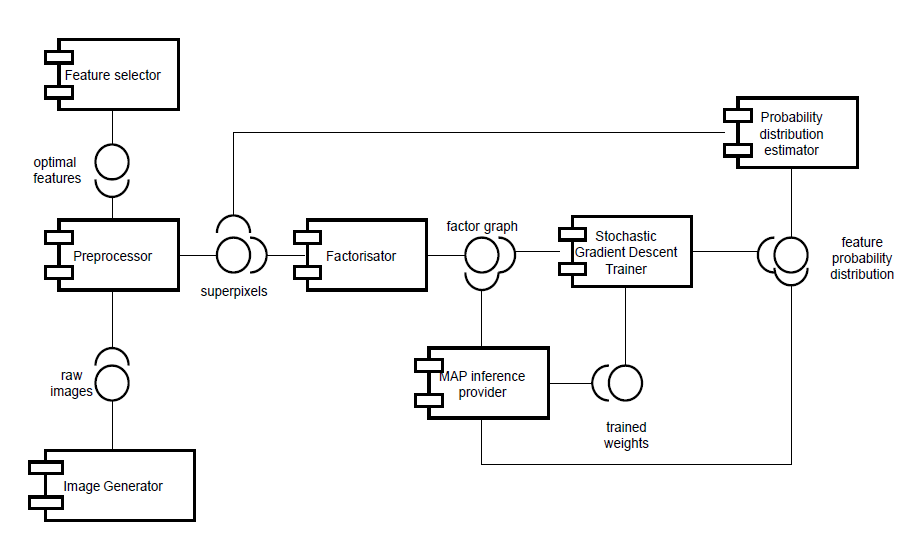
\includegraphics[width=\textwidth]{system_overview/component_diagram.png}
    \caption{Component diagram of the created semantic image segmentation system.}
    \label{fig:component_diagram}
\end{figure}


